\chapter{Elevation Map Generation}
\label{ch:elevation-map-generation}
When dealing with robot locomotion, the representation of the environment plays 
a fundamental role. It is, in fact, extremely important to properly
understand the structure of the world in order to safely make the robot move,
avoiding obstacles and dangerous zones, and to make it successfully complete 
its tasks. The world that surrounds the robot can be represented in many 
different ways; it is important to choose a proper representation to keep 
computational costs low and make to locomotion realizable.

In \textit{World of Stairs} scenarios, introduced in the previous chapter, the 
most efficient way to represent environments is by using elevation maps.
An elevation map is a grid that contains for each coordinate $(x, y)$ of the 
world its respective coordinate $z$. Hence, it can be seen as a function 
$\mathcal{M}_z$ such that, for each element $i$ of the grid,
$z_i = \mathcal{M}_z(x_i, y_i)$. This kind of representation allows the 
development of planners that quickly find plans to make robots move from a
position to another inside the world. 

This chapter introduces \texttt{elevation\_mapping}
\cite{Fankhauser2018ProbabilisticTerrainMapping}, the framework used in this 
thesis to generate elevation maps, which allow NAO to navigate in unknown 
environments (more precisely in \textit{World of Stairs} environments);
the ASUS Xtion Pro, an RGB-D sensor equipped on top of NAO, which has been 
used to send depth informaton to \texttt{elevation\_mapping}; 
the behaviour of the framework when a map is build using the ASUS Xtion Pro
placed on the head 
of NAO humanoid robot. The generated map is the one used in the experiment 
TODO and it is used by the footstep planner (Chapter
\ref{ch:rrt-based-footstep-planning}) to make NAO climb the stairs.

\section{Framework}
Todo (overview of elevation\_mapping). ROS.

\subsection{Definitions}
Todo (RFs).

\subsection{Map Update}
Todo (range measurements + robot motion).

\subsection{Map Fusion and Dynamic Environments}
Todo.

\section{ASUS Xtion Pro}
xtion (RGBD camera). ROS.
\begin{figure}
  \centering
  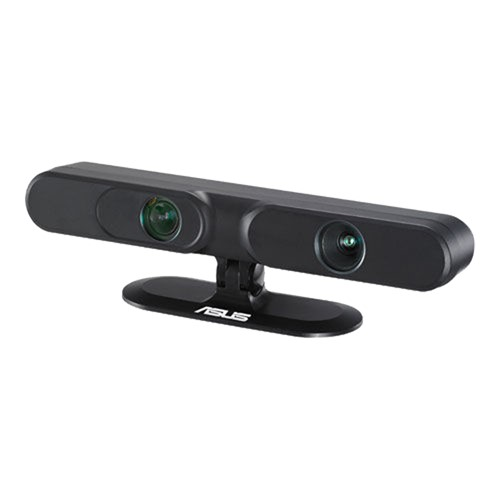
\includegraphics[width=0.5\textwidth]{figures/asus-xtion-pro.jpeg}
  \caption{The ASUS Xtion Pro is equipped with a depth sensor and it is 
      easily configurable to make it work with ROS. This simplifies the 
      integration with \texttt{elevation\_mapping} and, consequently, 
      the construction of a navigable map.}
  \label{fig:asus-xtion-pro}
\end{figure}

\section{World of Stairs}
(safe zone)
\begin{figure}
  \begin{subfigure}[b]{0.49\textwidth}
    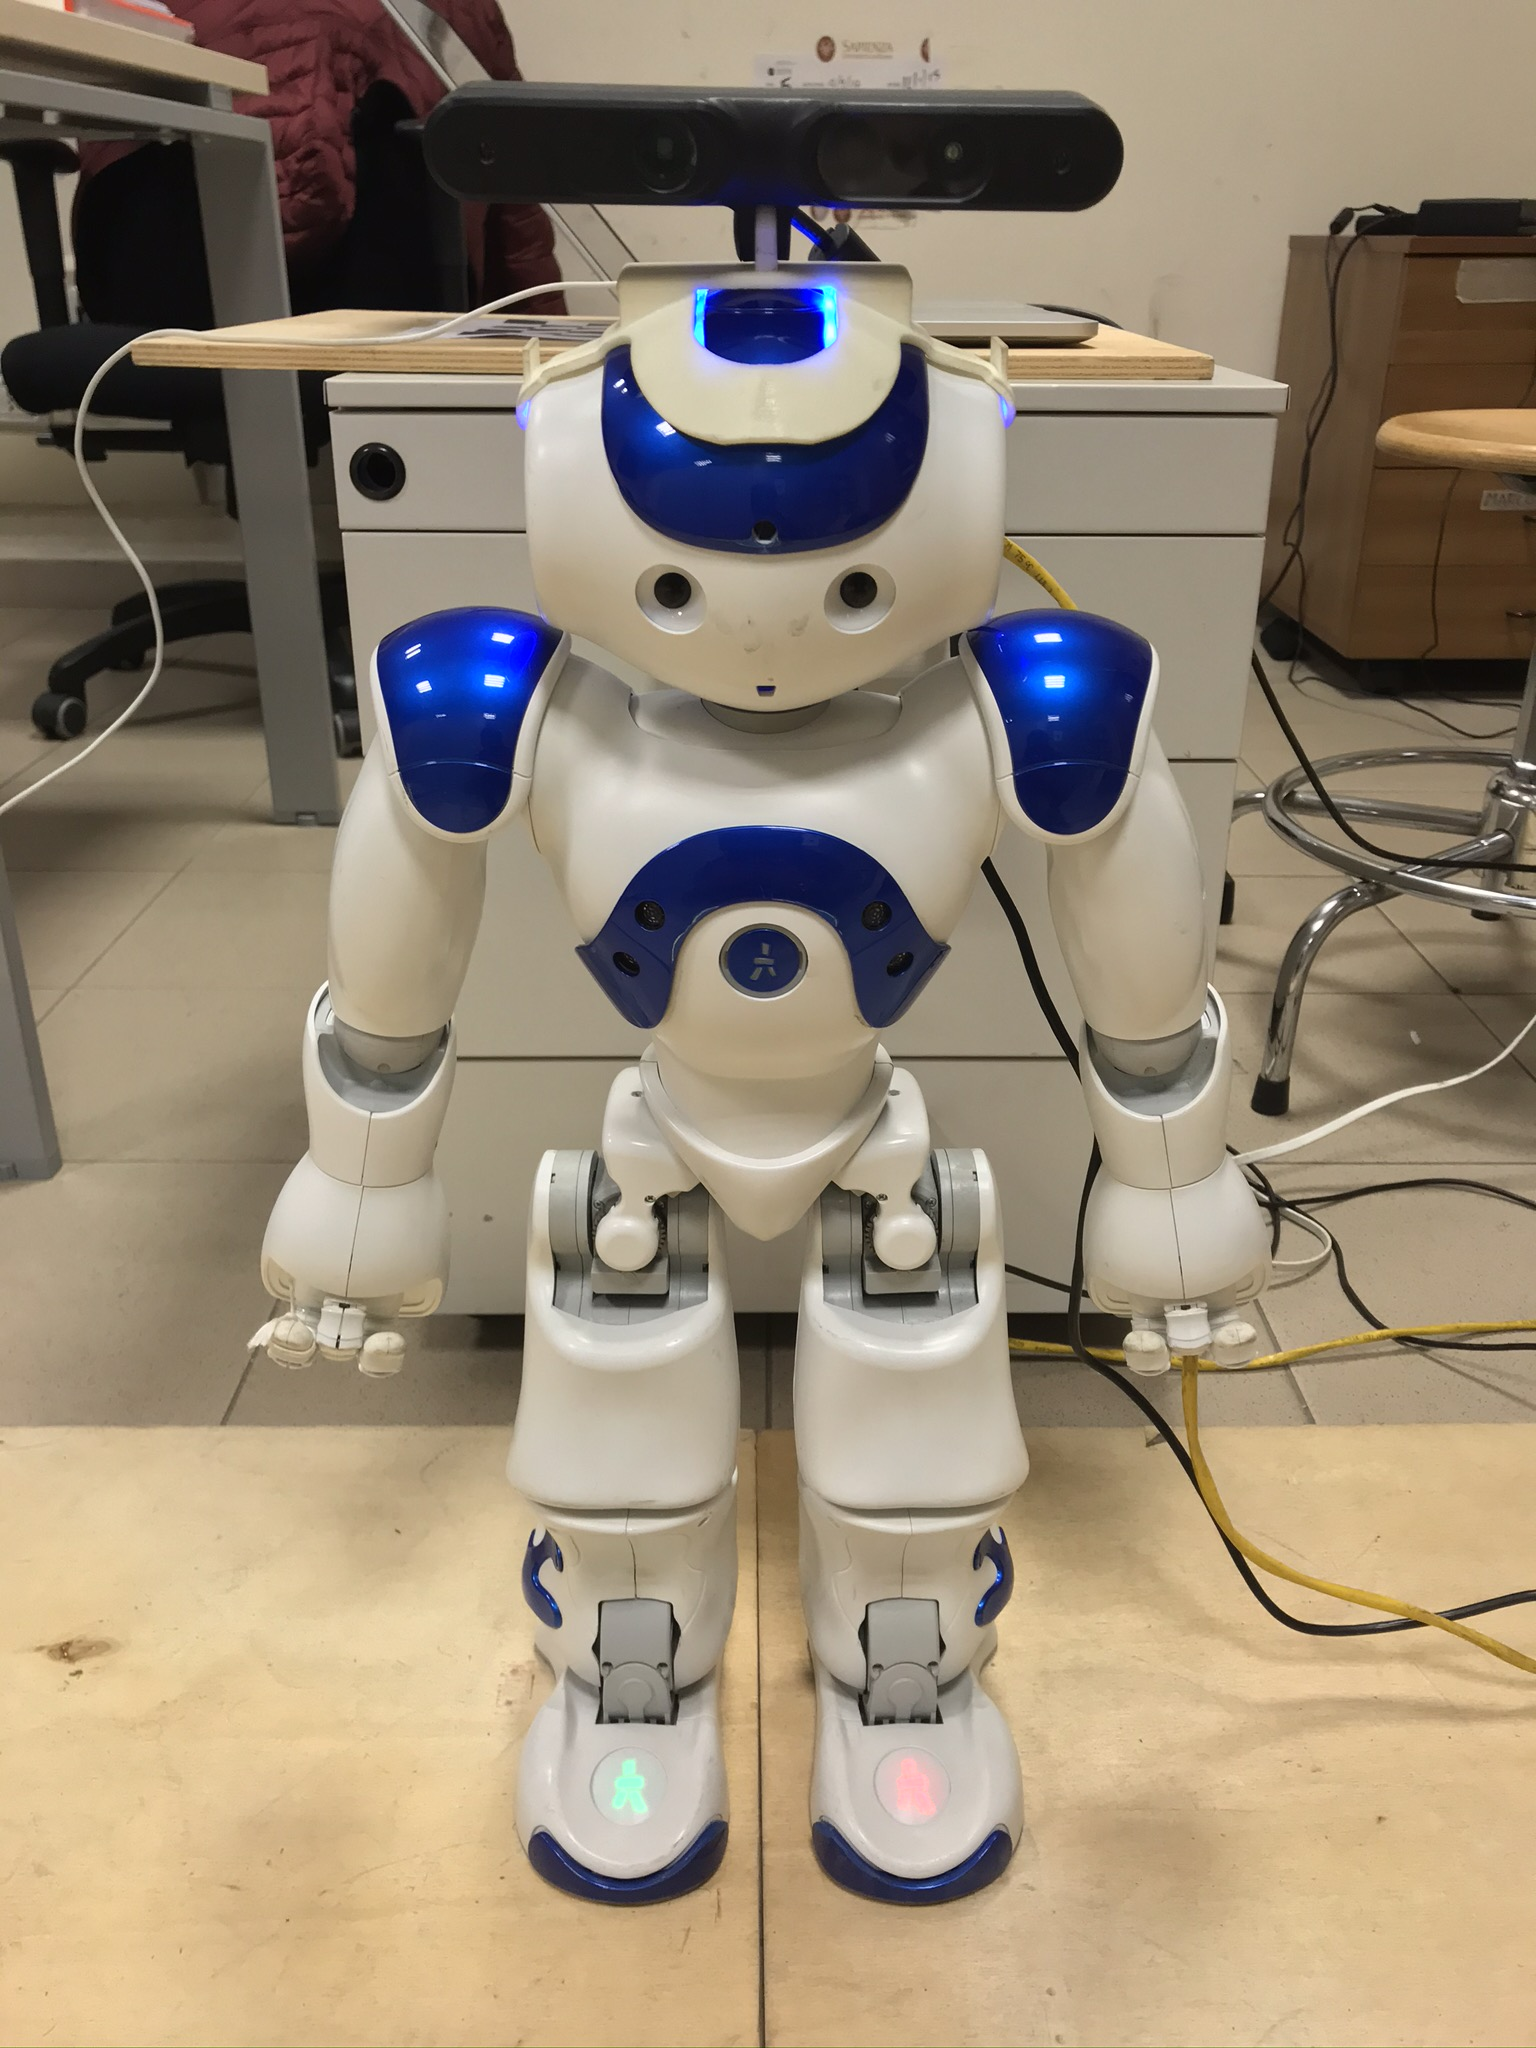
\includegraphics[width=\textwidth]{figures/NAO-with-xtion.JPEG}
    \caption{}
    \label{fig:nao-with-xtion}
  \end{subfigure}
  \hfill
  \begin{subfigure}[b]{0.49\textwidth}
    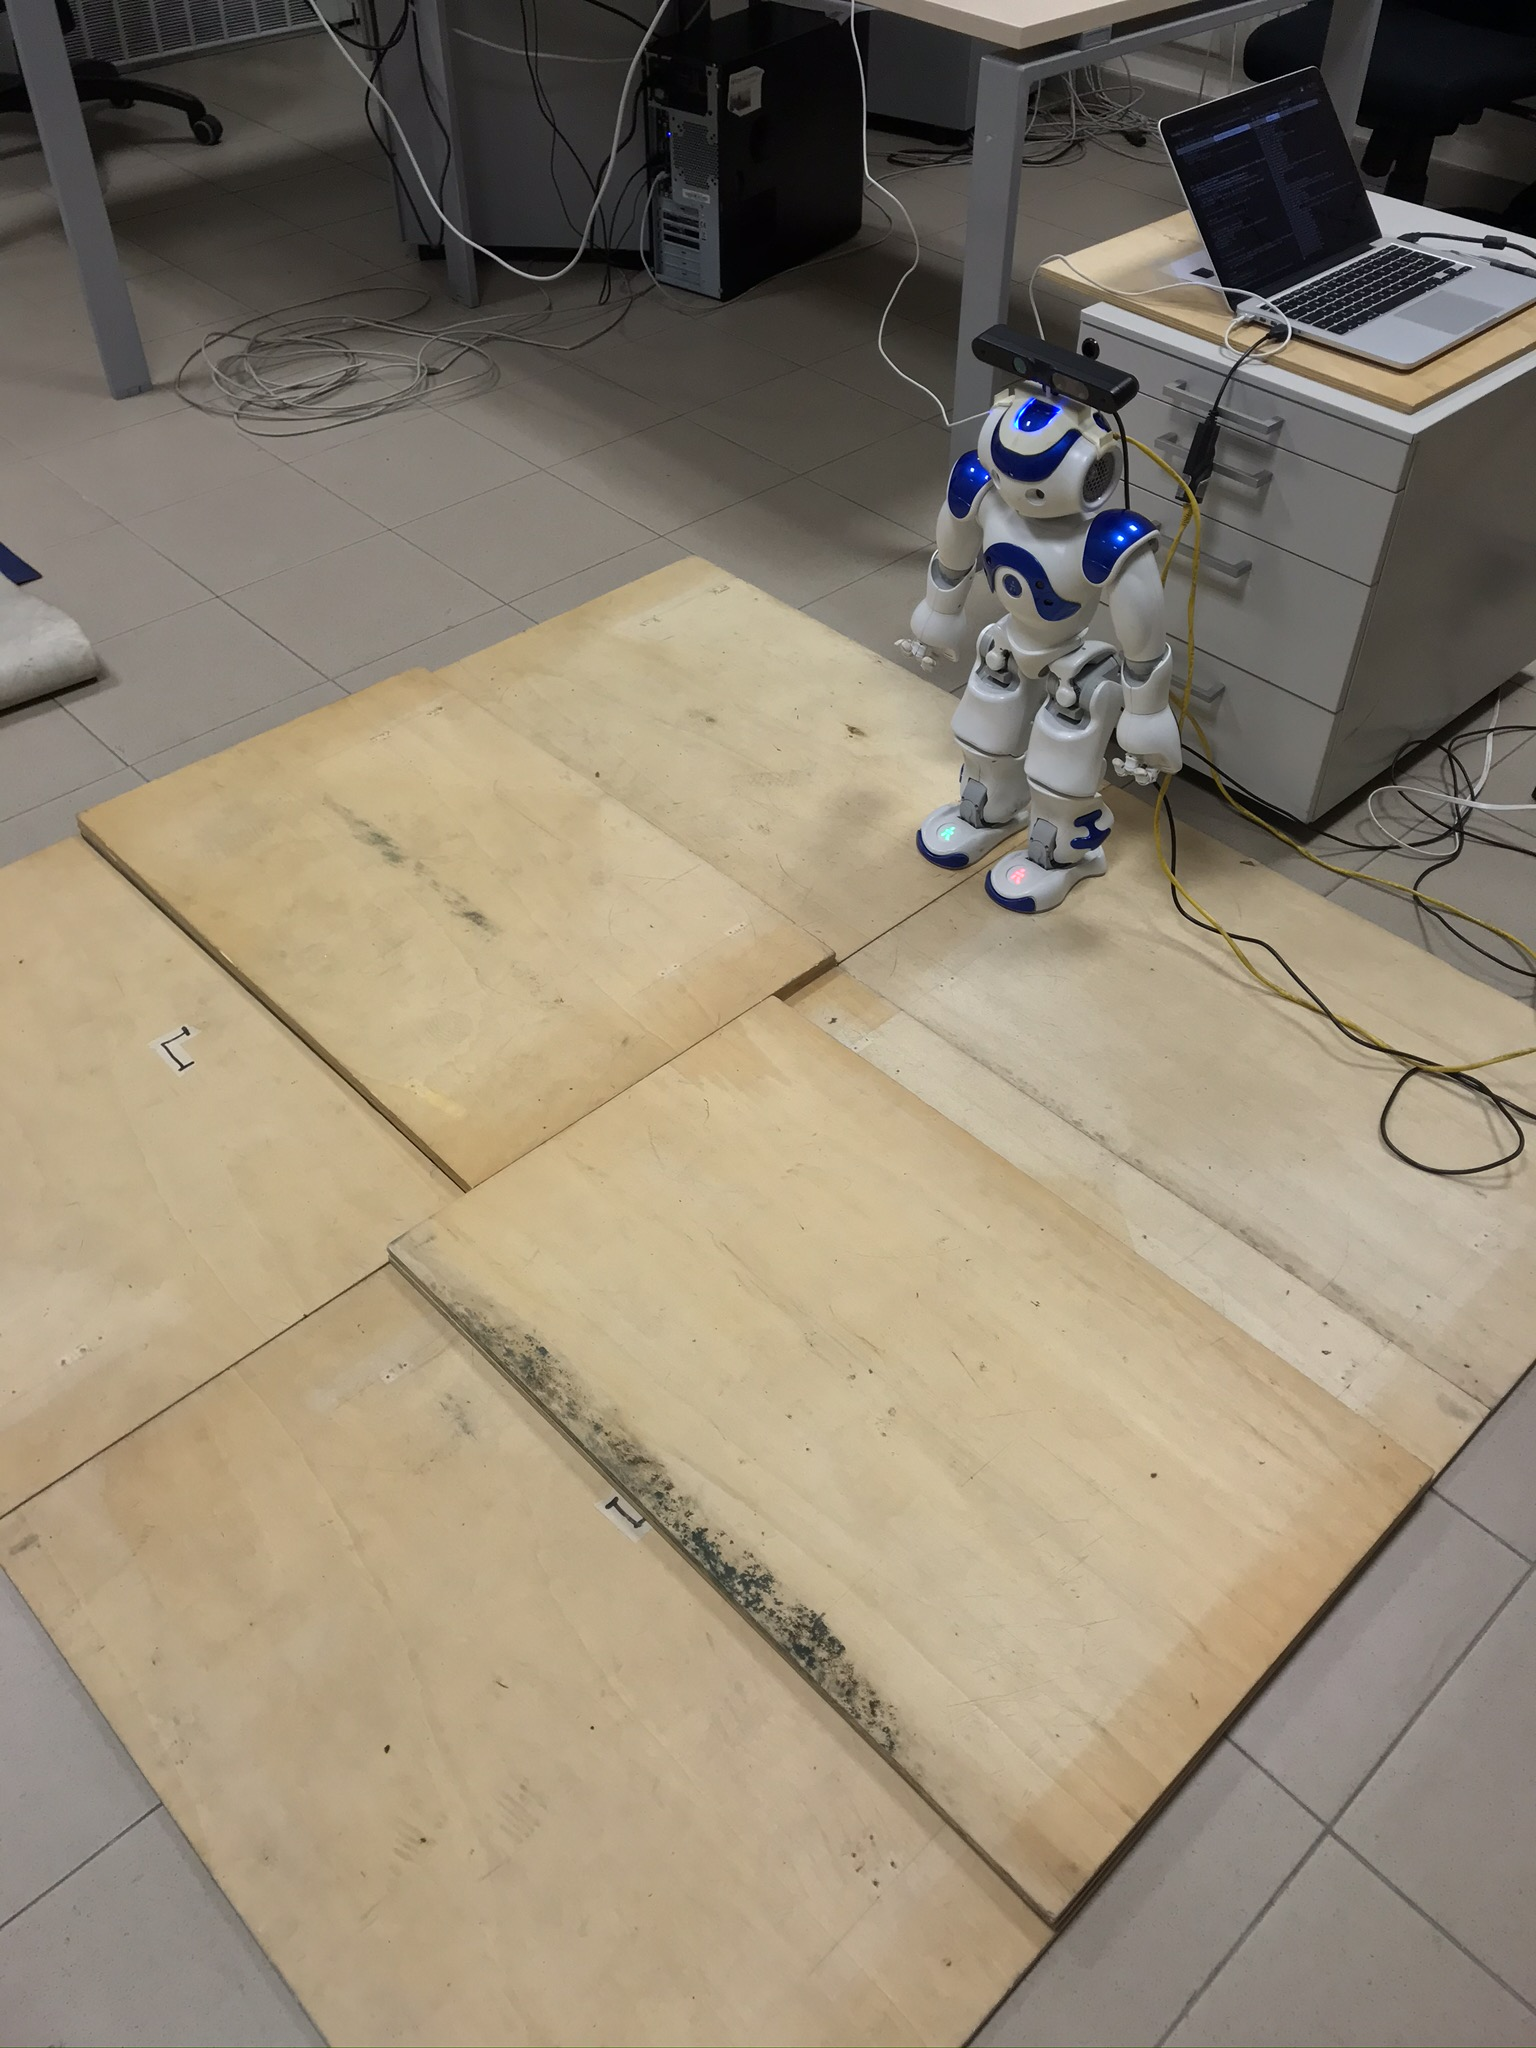
\includegraphics[width=\textwidth]{figures/NAO-with-xtion-full-env.JPEG}
    \caption{}
    \label{fig:nao-with-xtion-full-env}
  \end{subfigure}
  \caption{On the left, NAO humanoid robot with ASUS Xtion Pro placed on top.
      On the right, NAO humanoid robot in the environment described TODO, 
      right before starting the execution of the experiment.}
\end{figure}
\begin{figure}
  \centering
  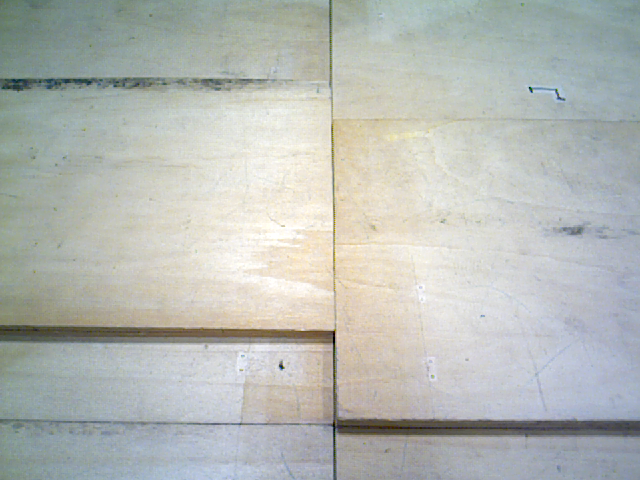
\includegraphics[width=0.85\textwidth]{figures/xtion_rgb_20cm.png}
  \caption{RGB image seen by the ASUS Xtion Pro placed on top of the robot.
      The corresponding depth image is sent to \texttt{elevation\_mapping}
      to build the map.}
  \label{fig:xtion-rgb-20cm}
\end{figure}
\begin{figure}
  \centering
  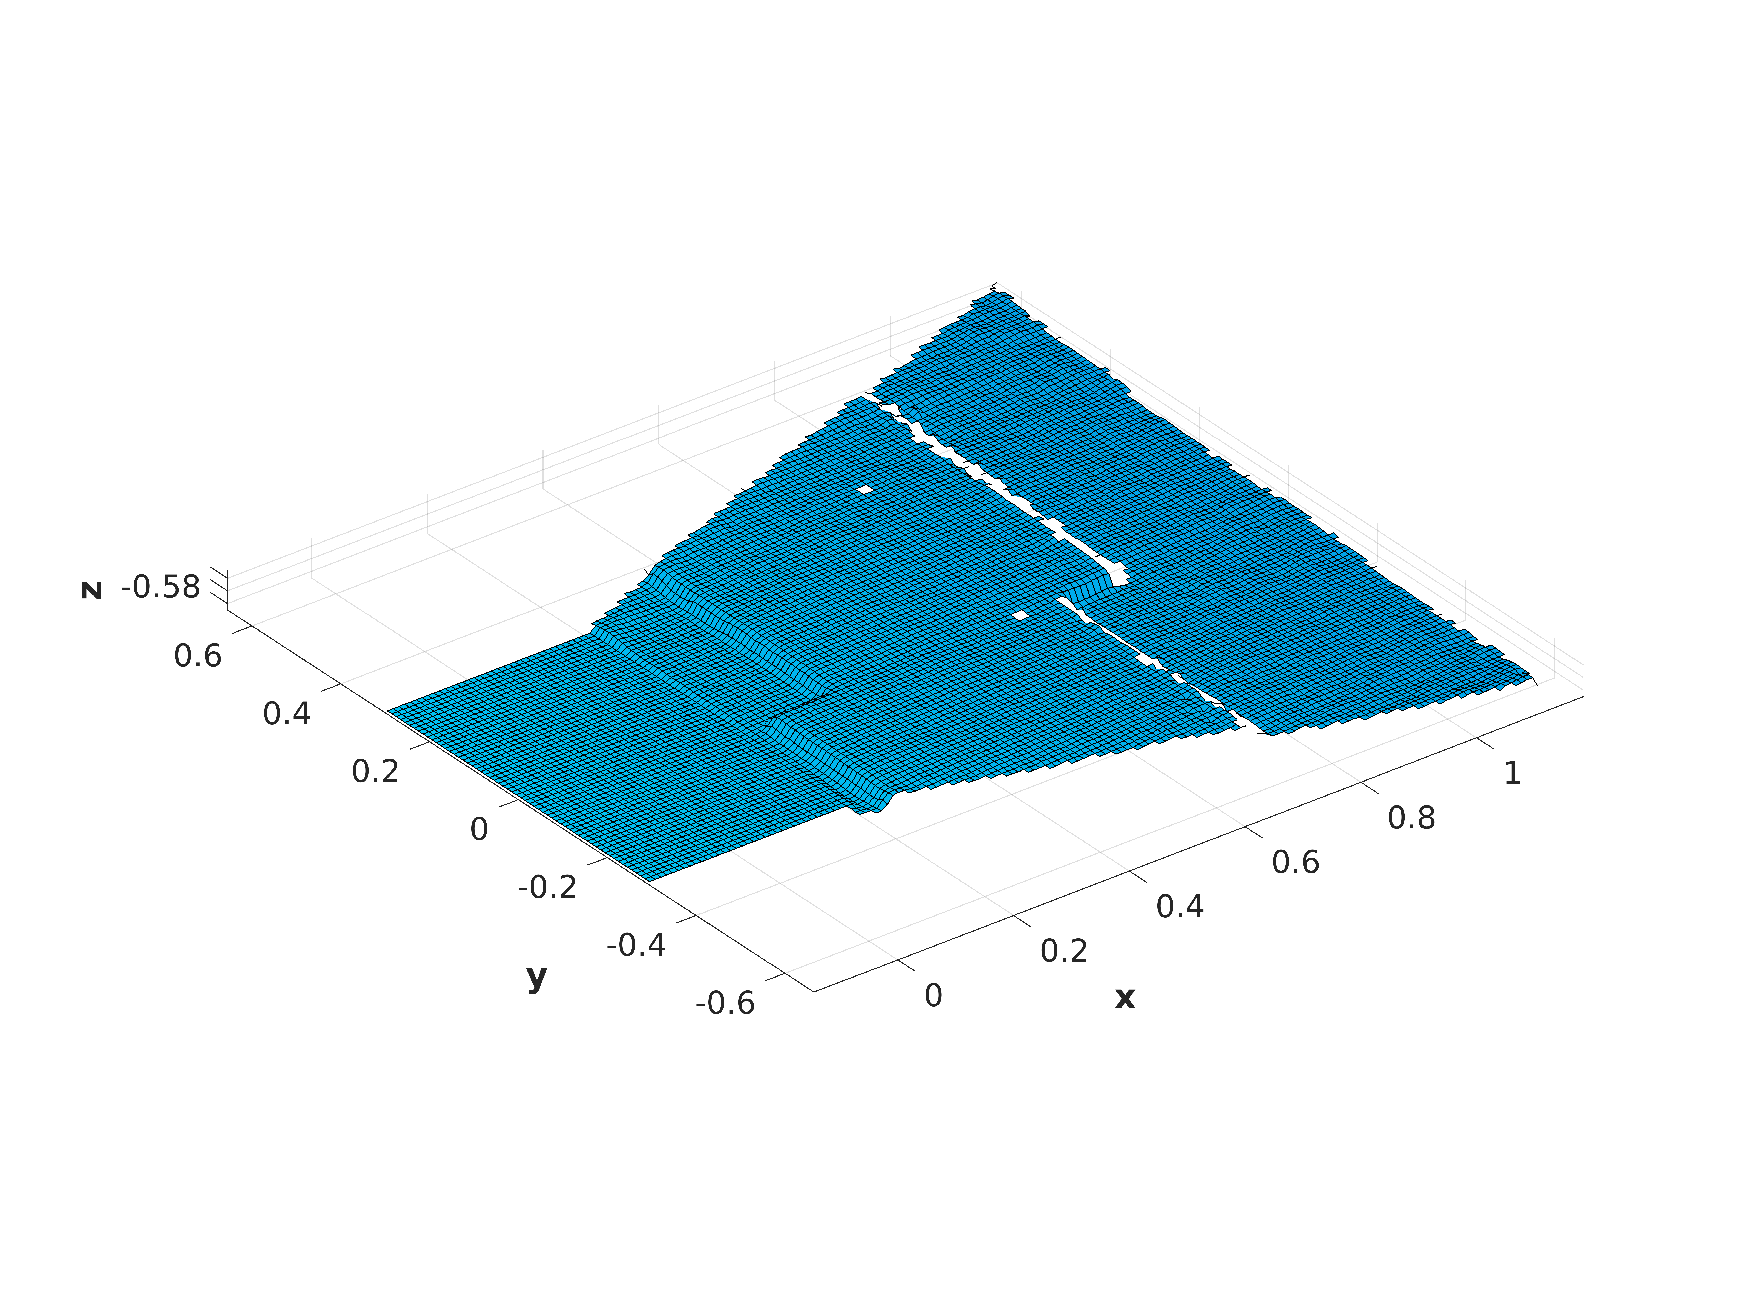
\includegraphics[width=\textwidth]{figures/onlymap-xtion-20cm.pdf}
  \caption{Elevation map build by \texttt{elevation\_mapping} for the 
      environment described TODO.}
  \label{fig:onlymap-xtion-20cm}
\end{figure}

